\section{Approach and Secret Weapon  }

\textbf{Naive Post-match. }

Our naive approach analyzed post-match data and tried to analyze whether a 
naive classifier could obtain a higher accuracy given all the information.  
Post-match data contains all the information about the match (except the winning 
team was withheld), including the number of kills on each team, the amount of minions 
that each team kind, the accumulation of gold for each player, etc.  We first pre-process 
the data to create a flattened vector representing the match.  
Given a set of training matches, we can apply the K-Clustering algorithm to train a 
set of \"features\" based on these training matches.  Using Orthogonal Matching Pursuit, we can then create a sparse code representation for these training matches.  
We can then train an SVM classifier using these sparse codes and the 
match outcomes to use for predicting the outcomes of future matches.  
We can test the SVM model by repeating the same process with a new testing data set.  Given that this approach has access to all the post-match data, 
we expect some variables to be highly correlated with the match 
outcome (more kills or more gold probably implies victory).

\textbf{Pre-match. }

Our next approach attempts to analyze only the pre-match data in order to create 
a classifier for the match's outcome.  In this case, we only examine variables 
intrinsic to the game itself rather than the performance of the teams and members 
during the match.  An example of an in-game intrinsic is if the team that has a 
certain champion (or set of champions) always seems 
to win or lose.  In this case, we would ignore the statistics of the matches 
actual performance, and instead try to discover whether there are certain inherent 
characteristics of the game that lead to certain advantages.  Our work-flow is similar 
to the one used in the post-game technique.

\textbf{Secret Weapon: Match Histories.  }
Our goal was to be able to predict which team would win a certain match before it occurs. 
We could therefore leverage the knowledge of matches in the past, as well as the pre-game 
information for this certain game.  Our naive post-match method is too constricting, 
requiring us to know the entire post-match data in order to classify the winner.  Our pre-match 
method is not optimal, since it forgoes all the important information that can be extracted 
from past match histories.  Match histories can generate useful information such as 
overall skill level, trends in some of the previously mentioned features, 
affinities for particular champions, and most importantly relationships with other 
players.  Match histories give deeper insight between the possible synergy between 
players that are matched together.  

Analyzing the recent match histories for each of the players in the game 
(five on each team, ten total) would be helpful to build a sophisticated model for the predictor.  
We limit match history calculations to the most recent 150 matches in order to 
minimize data explosion.  Even with this 
limitation, incorporating match histories significantly inflates the amount of 
data required and processed to analyze a single match.  
For example, to process a single match, we now require data from $1 \mbox{ match} * 10 \frac{\mbox{players}}{\mbox{match}} * 150 \frac{\mbox{games}}{\mbox{player}} = 1500 \mbox{ games}$ to be analyzed. 

\textbf{Data Wrangling. }

Match histories are most useful when you can determine relationships between the players. 
Single occurences of each relationship would be of little help (i.e., Player 1 and 2 show up on the same or different team only once).
Moreover, the large data explosion that occurs when gathering match history data makes this scenario even less desirable.  However, by carefully selecting the proper subset of matches to analyze, we can increase the overlap of players between matches. League of Legends has a division system (divisions which are called Bronze, Silver, Gold, Platinum, Diamond, Master, and Challenger) which breaks down players based on an ELO-type of rating. The trend seems to show that the higher the division, the less players there are in that division. 

%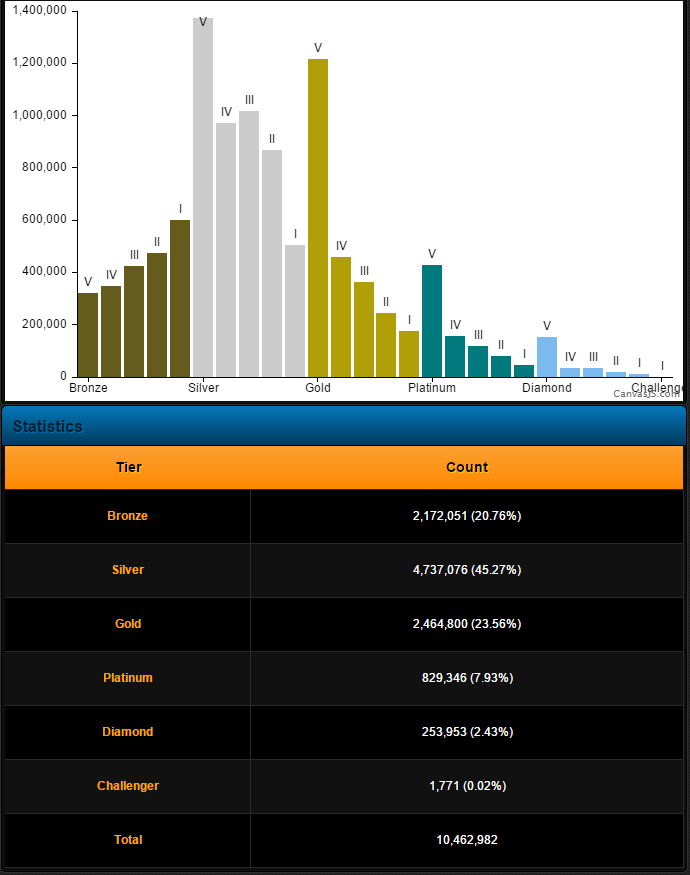
\includegraphics[scale=.5]{figures/rankedbreakdown}

Due to this system, people in the higher brackets are matched with the same people much more frequently. We can thus increase the effectiveness of our computation by selecting games of Challenger players. This was seen as in our analysis of 543 games, we archived the history for 787 unique players. This ratio is $\frac{787}{543} = 1.44$ players per game, which is far better than the ratio of 10 unique players per game which we would expect if we looked at a completely random match. 

After acquiring the player histories, the data needs to be pre-processed and converted into a format that can be inputted into an ML model.  As with our previous convention, we want to create a vector (or a matrix in this case, due to multiple matches in a match history) to represent each match. 

Although applying PCA would be ideal for reducing the dimensions of the data and maintaining variance, we explicitly chose a relatively dense set of features based on 
specific domain knowledge of the game.  ("Kills", "Deaths", "Assists", "GoldEarned", "DamageToChampions", "DamageOverall", "GamesPlayed", "Wins". This is a good introductory feature set, as though it lacks some of the more complex to express features which mirror complex strategies in the game, it contains the basics.) 

Once these features were extracted and transformed into a CSV format easily consumable by the sklearn python module, I split the data into a training and testing set and fed it into a SVM model and a Random Forest Classifier. No sparsifying of the dataset was one before-hand, as the set of features is dense. 